% Output-levers ladder for Ch17 ("Shaping Output — Structured & Reliable").
% Standalone TikZ; compiled by `book-scaffold build-figures` via pdflatex -> pdftocairo -> SVG.
% The four levers that force machine-readable output, strongest guarantee (top) to lightest
% weight (bottom): structured outputs / strict (grammar-constrained guarantee, with caveats),
% tool_use + tool_choice (forces the call), validation + retry (recover path), prompt-asked JSON
% (no guarantee). Each rung is annotated with what it actually guarantees.
\documentclass[tikz,border=4mm]{standalone}
\usepackage{tikz}
\usetikzlibrary{positioning, arrows.meta, calc}

\begin{document}
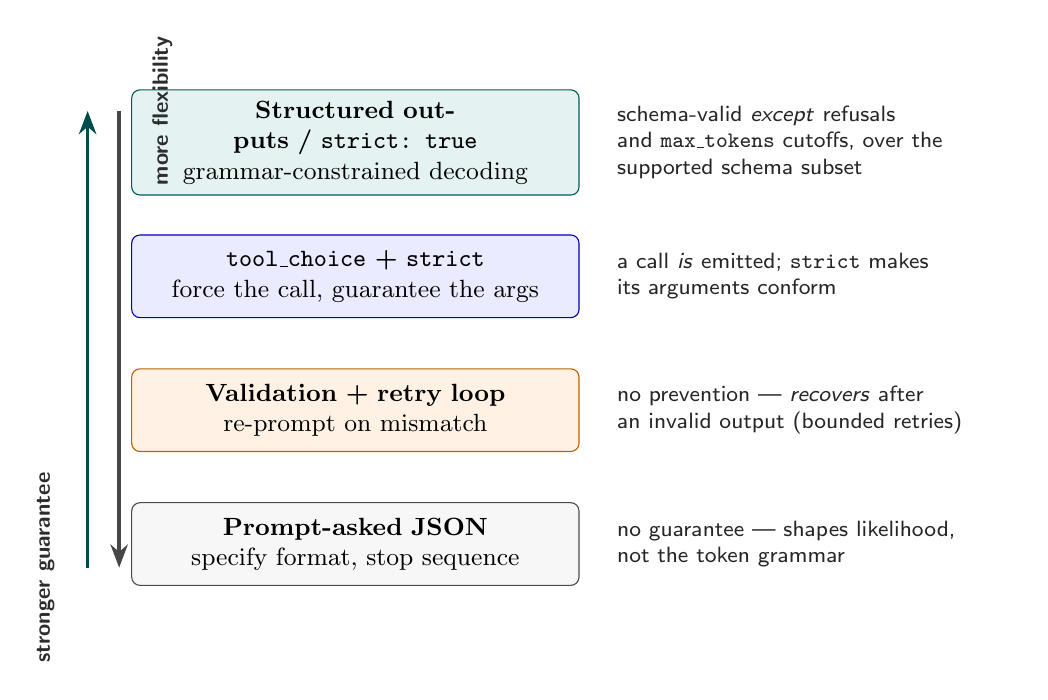
\begin{tikzpicture}[
  font=\sffamily,
  rung/.style={draw=gray!55!black, rounded corners=3pt, align=center,
    text width=5.4cm, minimum height=1.05cm, inner sep=4pt, font=\small},
  strong/.style={rung, draw=teal!70!black, fill=teal!10},
  mid/.style={rung, draw=blue!70!black, fill=blue!8},
  recover/.style={rung, draw=orange!75!black, fill=orange!10},
  light/.style={rung, draw=gray!60!black, fill=gray!6},
  guar/.style={font=\sffamily\footnotesize, text=gray!30!black, anchor=west, align=left,
    text width=5.0cm},
  axlabel/.style={font=\sffamily\bfseries\footnotesize, text=gray!35!black, rotate=90, anchor=south}
]

% rungs, strongest guarantee at the top
\node[strong]  (so)  at (0, 0)    {\textbf{Structured outputs / \texttt{strict: true}}\\grammar-constrained decoding};
\node[mid]     (tc)  at (0, -1.7)  {\textbf{\texttt{tool\_choice} + \texttt{strict}}\\force the call, guarantee the args};
\node[recover] (rt)  at (0, -3.4)  {\textbf{Validation + retry loop}\\re-prompt on mismatch};
\node[light]   (pj)  at (0, -5.1)  {\textbf{Prompt-asked JSON}\\specify format, stop sequence};

% annotations to the right — what each guarantees
\node[guar] at (3.2, 0)    {schema-valid \emph{except} refusals\\and \texttt{max\_tokens} cutoffs, over the\\supported schema subset};
\node[guar] at (3.2, -1.7)  {a call \emph{is} emitted; \texttt{strict} makes\\its arguments conform};
\node[guar] at (3.2, -3.4)  {no prevention --- \emph{recovers} after\\an invalid output (bounded retries)};
\node[guar] at (3.2, -5.1)  {no guarantee --- shapes likelihood,\\not the token grammar};

% guarantee-to-flexibility axis on the left
\draw[-Stealth, very thick, draw=teal!60!black] (-3.4,-5.4) -- (-3.4,0.4);
\node[axlabel] at (-3.7,-5.4) {stronger guarantee};
\draw[-Stealth, very thick, draw=gray!55!black] (-3.0,0.4) -- (-3.0,-5.4);
\node[font=\sffamily\bfseries\footnotesize, text=gray!35!black, rotate=90, anchor=north]
  at (-2.7,0.4) {more flexibility};

\end{tikzpicture}
\end{document}
